\documentclass{article}

% Define margins
\setlength{\topmargin}{-1.0cm}
\setlength{\oddsidemargin}{0.1cm}
\setlength{\textwidth}{16.5cm}
\setlength{\textheight}{23.0cm}

% Packages
\usepackage{url}
\usepackage[hidelinks]{hyperref}
\usepackage{subfig}
\usepackage{graphicx}

% Color
\usepackage{xcolor}
\newcommand{\magenta}[1]{\textcolor{magenta}{#1}}
\newcommand{\red}[1]{\textcolor{red}{#1}}
\newcommand{\blue}[1]{\textcolor{blue}{#1}}
\newcommand{\green}[1]{\textcolor{green}{#1}}



\begin{document}
	\noindent\huge \textbf{Research Statement} \\
	\vspace{0.1em}\\
	\Large \textbf{Bishwamittra Ghosh}
		
	\normalsize
	\noindent Ph.D.\ Candidate\\
	School of Computing\\
	National University of Singapore (NUS)\\
	\blue{\url{https://bishwamittra.github.io}}



	\paragraph{}
	My research interest is in fairness and interpretability in machine learning applied in safety-critical domains. Traditional machine learning, specifically deep learning, is infamous for its unfair/biased prediction towards certain demographic groups, and for providing uninterpretable black-box predictions. To meet these challenges, I design scalable algorithms to verify and understand the bias of machine learning classifiers and to learn interpretable classifiers. In my research, I closely integrate automated reasoning, formal methods, and statistics with fairness and interpretability in machine learning.
	
	
	
	In my doctoral dissertation, I have focused on the safety-critical aspects of machine learning: \textbf{fairness} and \textbf{interpretability}. Particularly, we have proposed algorithmic frameworks for \emph{verifying the fairness of classifiers}~\cite{ghosh2021justicia,ghosh2022algorithmic}, \emph{identifying sources of the unfairness of classifiers}~\cite{ghosh2022how}, and \emph{designing efficient interpretable classifiers}~\cite{ghosh22efficient,ghosh2019incremental,ghosh2020classification}. Fairness verification provides a formal certificate of whether a classifier achieves the desired level of fairness on specified data distribution. For identifying the sources of unfairness, we compute fairness influence functions of input features as their contribution towards the bias of the classifier. In interpretable machine learning, we efficiently learn interpretable rule-based classifiers alternative to black-box classifiers. In particular, we propose a scalable learning framework through incremental learning to learn accurate and small interpretable classification rules while enabling learning on large datasets.
	
	
	My research has thrived through multiple collaborations and internships in industry and academia. Beyond fairness and interpretability, I have collaborated on solving research problems on  group testing~\cite{ciampiconi2020maxsat} and social-spacial group queries~\cite{ghosh2018flexible,apon2021social}. Our works have been published at premier conferences and journals in artificial intelligence and machine learning (AAAI-$ 2022, 2021, 2020 $, JAIR-$ 2022 $, ECAI-$ 2020 $, AIES-$ 2019 $) and databases (VLDB-$ 2018 $, TSAS-$ 2022 $).
	
	
	
	
	
	\section*{Dissertation Summary}
	
	\subsection*{Research Thrust 1: Fairness in Machine Learning}
	
	Fairness in machine learning centers on detecting and mitigating bias towards different sensitive groups in the data induced by the classifier. In recent years, fairness literature is bestowed with multiple fairness definitions and algorithms to quantify and improve fairness. The goal of our research is to assess the fairness claim of a classifier by proposing a formal fairness verification framework. Furthermore, we dive into understanding the sources of unfairness to develop better fairness algorithms in the future.
	
	\paragraph{Probabilistic Fairness Verification.} Given the distribution of input features and a classifier trained on samples from the same distribution, our probabilistic fairness verifier, called $ \mathsf{Justicia} $, certifies whether the classifier achieves the desired level of fairness according to a group fairness metric~\cite{ghosh2021justicia}. Being a probabilistic verifier, $ \mathsf{Justicia} $ robustly estimates the bias of a classifier in contrast to measuring bias on a finite dataset (Figure~\ref{fig:sample-size})\textemdash one popular notion of bias is statistical parity, which is the difference between the maximum and minimum conditional probability of a binary classifier's positive prediction over all sensitive groups. Based on a stochastic satisfiability (SSAT) formulation, $ \mathsf{Justicia} $ is the \emph{first fairness verifier for compound sensitive groups} (combination of multiple sensitive features, such as Black-female and White-male), as highlighted in Figure~\ref{fig:protected_groups}. Methodologically, $ \mathsf{Justicia} $ encodes the classifier as a propositional formula in Conjunctive Normal Form (CNF), and verifies fairness by solving weighted model counting problems, specifically through an SSAT reduction. For example, the maximum conditional probability of the classifier's positive prediction is equal to the solution of an SSAT formula, where the sensitive features are assigned \emph{existential} quantifiers to derive their \emph{maximal} assignment such that the satisfying probability of the CNF classifier becomes maximum for random values of non-sensitive features. Similarly, to compute the minimum conditional probability of the classifier's positive prediction, it suffices to assign sensitive features with \emph{universal} quantifiers to optimize for their \emph{minimal} assignment. Consequently, $ \mathsf{Justicia} $ benefits from future improvement in SSAT solving, as the modeling of fairness verification into SSAT is separate from solving SSAT formulas. Also, multiple group fairness metrics can be verified in the same SSAT formulation by imposing additional conditionals on the CNF classifier. In experiments, $ \mathsf{Justicia} $ verifies the fairness of decision tree and CNF classifiers with superior performance in both accuracy and scalability than existing SMT or sampling-based verifiers. 
	
	
	\paragraph{Scalable Fairness Verification with Feature Correlations.} In our follow-up work on probabilistic fairness verification, we specifically focus on linear classifiers by proposing a verifier $ \mathsf{FVGM} $~\cite{ghosh2022algorithmic}. We improve both the scalability (Figure~\ref{fig:scalability_exp}) and accuracy of verification by proposing a stochastic subset-sum problem ($ \mathsf{S3P} $) based reduction and enabling feature correlations represented as a Bayesian Network. Theoretically, $ \mathsf{S3P} $ achieves a pseudo-polynomial complexity based on dynamic programming in contrast to the $ \mathrm{NP}^{\mathrm{PP}} $ hardness of SSAT. Also, $ \mathsf{S3P} $ reduction for linear classifiers is efficient as it avoids the expensive pseudo-Boolean to CNF encoding in $ \mathsf{Justicia} $~\cite{ghosh2021justicia}. Furthermore, $ \mathsf{FVGM} $ demonstrates significantly higher accuracy than prior verifiers because of considering correlated features. In applications of fairness verifiers, $ \mathsf{FVGM} $ tests the effectiveness of multiple fairness enhancing and fairness attack algorithms on popular datasets in fairness literature.
	
	
	\paragraph{Fairness Influence Functions.} Our next research quest is to \emph{quantify the influence of different features on the incurred bias of a classifier on a dataset}~\cite{ghosh2022how}. To this end, we propose a framework of Fairness Influence Function (FIF), and compute it as a scaled difference of the conditional variances in the classifier’s prediction. Based on global sensitivity analysis (GSA), we instantiate an algorithm, $ \mathsf{FairXplainer} $, that uses variance decomposition among the subset of features and a local regressor to compute FIFs accurately, while also capturing the intersectional effects of the features. Our experimental analysis validates that FairXplainer captures the influences of both individual features and higher-order feature interactions, estimates the bias more accurately than existing local explanation methods (Figure~\ref{fig:estimation_error}), and detects the increase/decrease in bias due to fairness affirmative/punitive actions in the classifier.
	
	
	\begin{figure*}[t!]
		\begin{minipage}{0.45\textwidth}
			\centering
			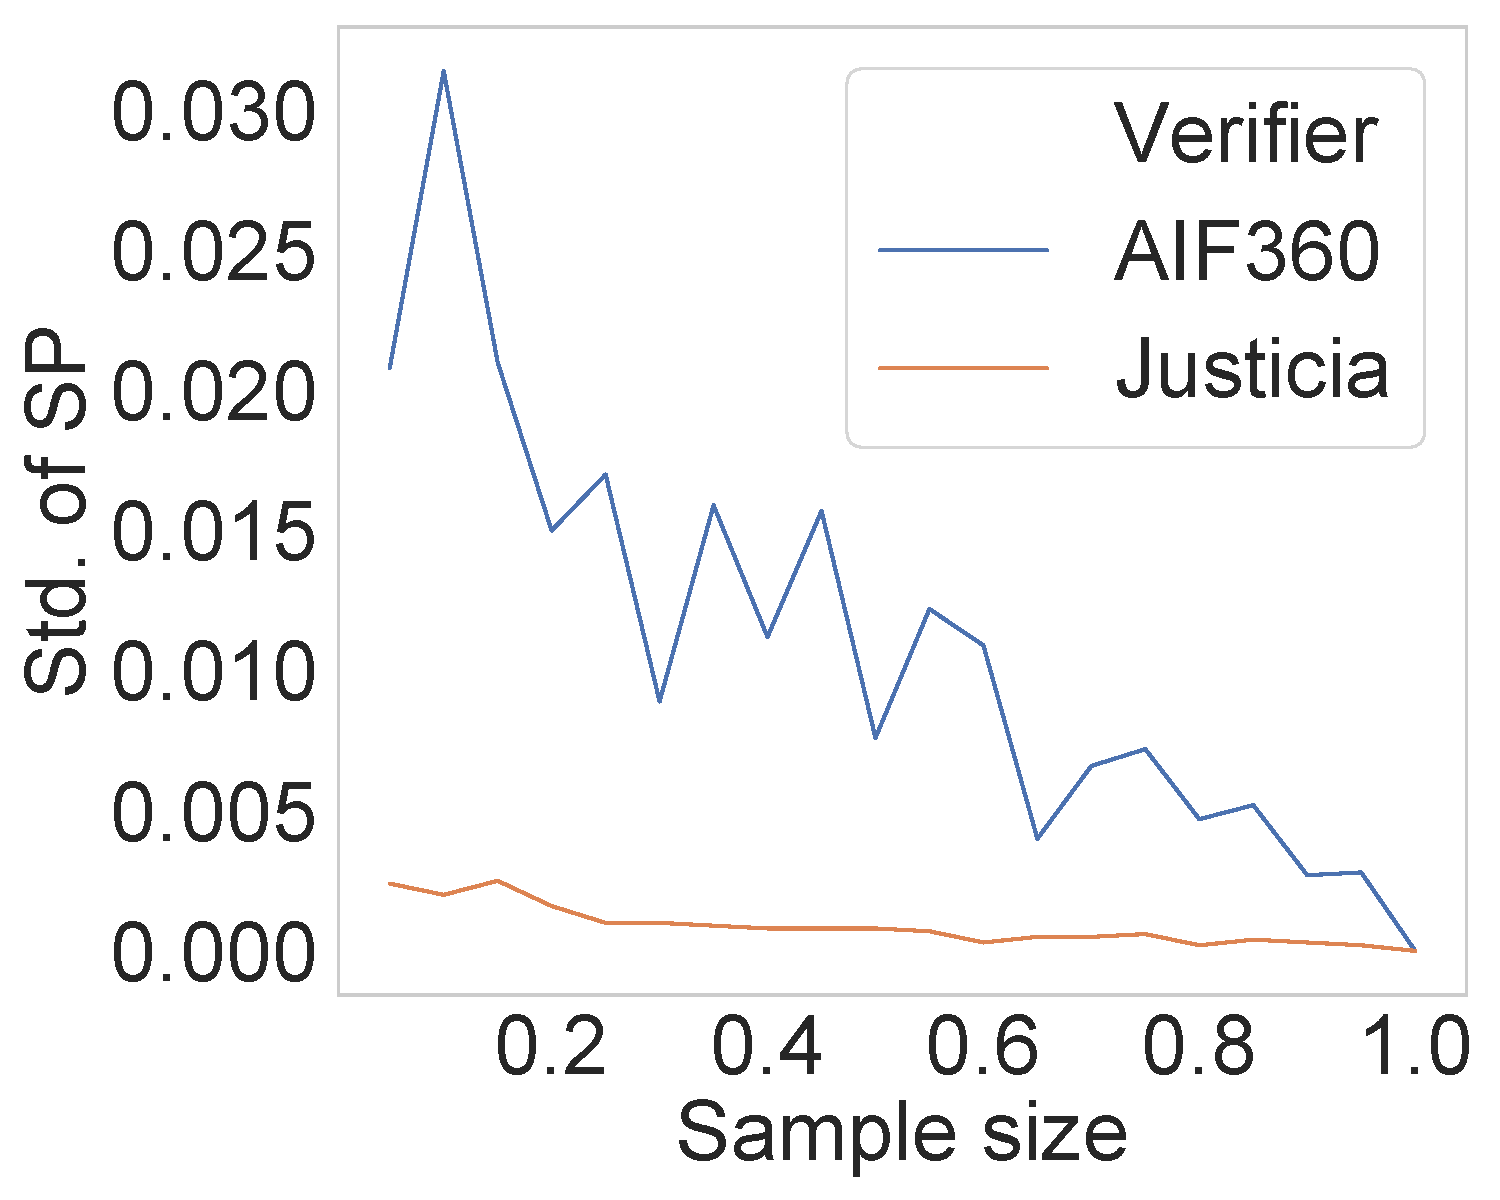
\includegraphics[scale=.18]{figures/sampling_SPD_after_Adult_rw_LR_race.pdf}
			\caption{Standard deviation in the estimation of statistical parity (SP)  for different sample sizes (sample size $ = 1 $ denotes the entire dataset). Probabilistic verifier $ \mathsf{Justicia} $ is more robust with the variation in sample size than AIF360 estimating statistical parity on a finite dataset. }
			\label{fig:sample-size}
		\end{minipage}\hfill
		\begin{minipage}{0.48\textwidth}
			\centering
				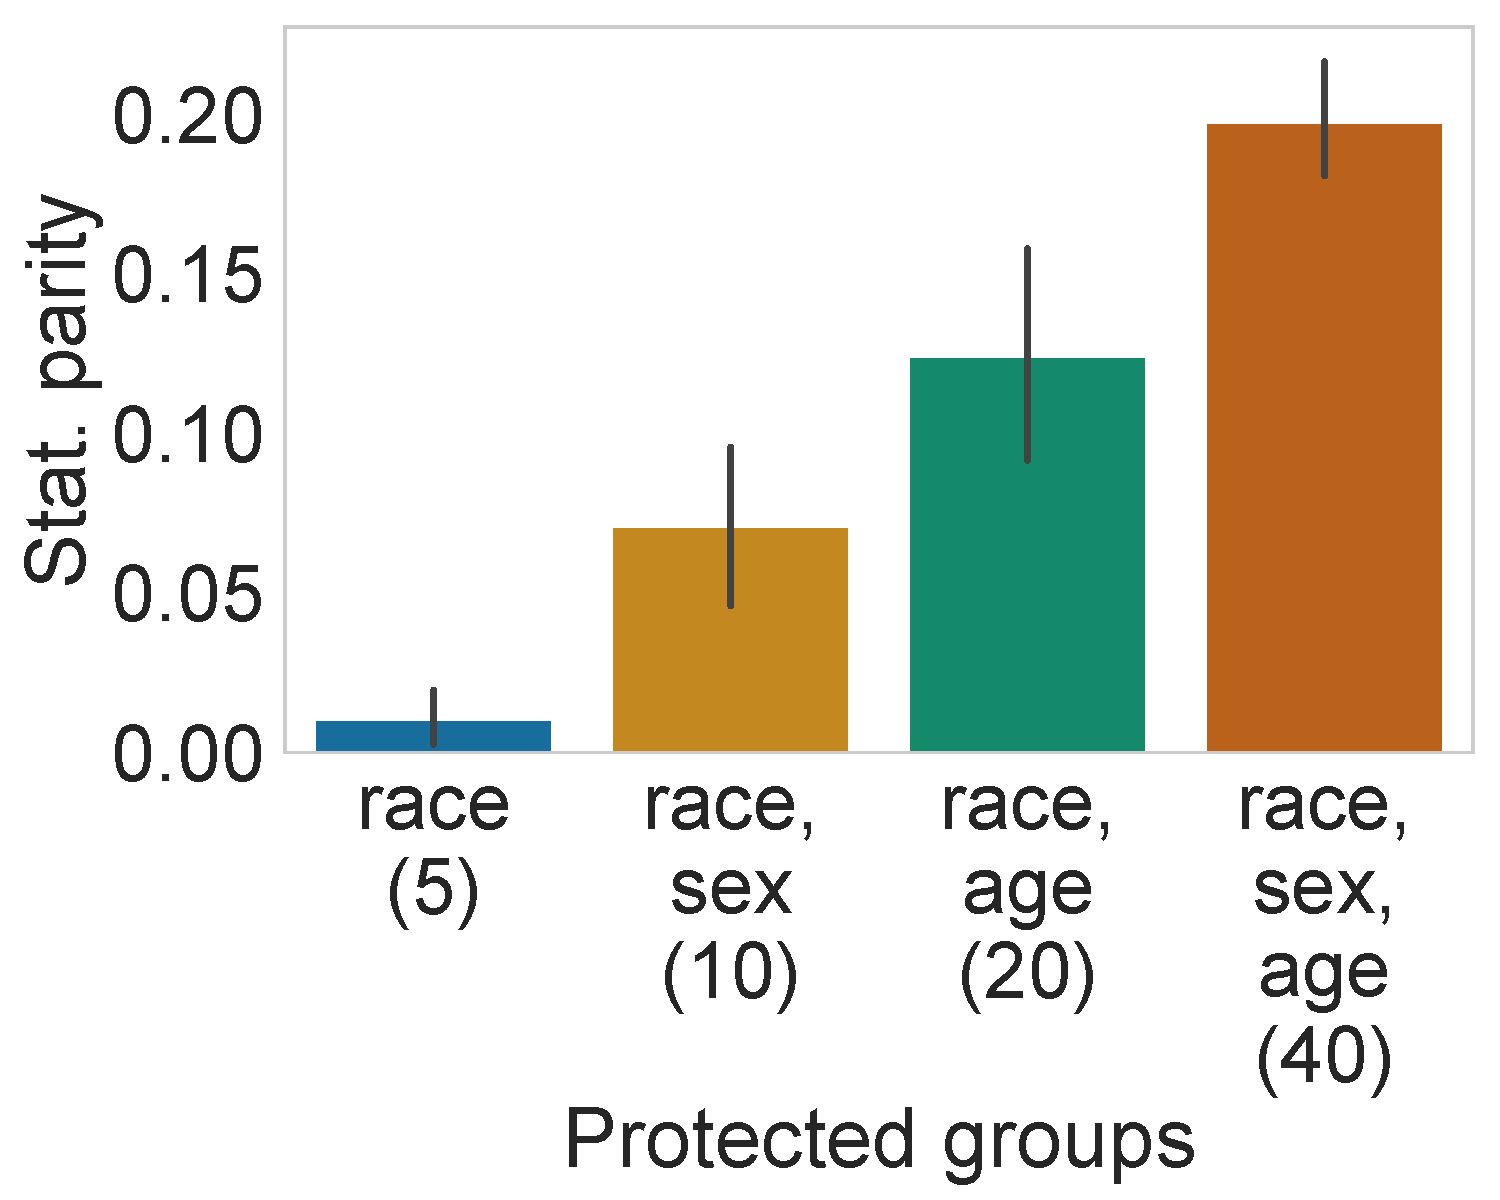
\includegraphics[scale=.18]{figures/sensitive_attribute_race_spd_Adult_DT_RE.pdf}
			\caption{Statistical parity verified by $ \mathsf{Justicia} $ for different sensitive/protected groups in the Adult dataset. The number within parenthesis in the xticks denotes total compound sensitive groups. The classifier demonstrates more unfairness (higher statistical parity) when considering more groups.}
			\label{fig:protected_groups}
		\end{minipage}
	\end{figure*}
	
	
	
	\begin{figure}
		\begin{minipage}{0.47\textwidth}
			\centering\begin{center}		
			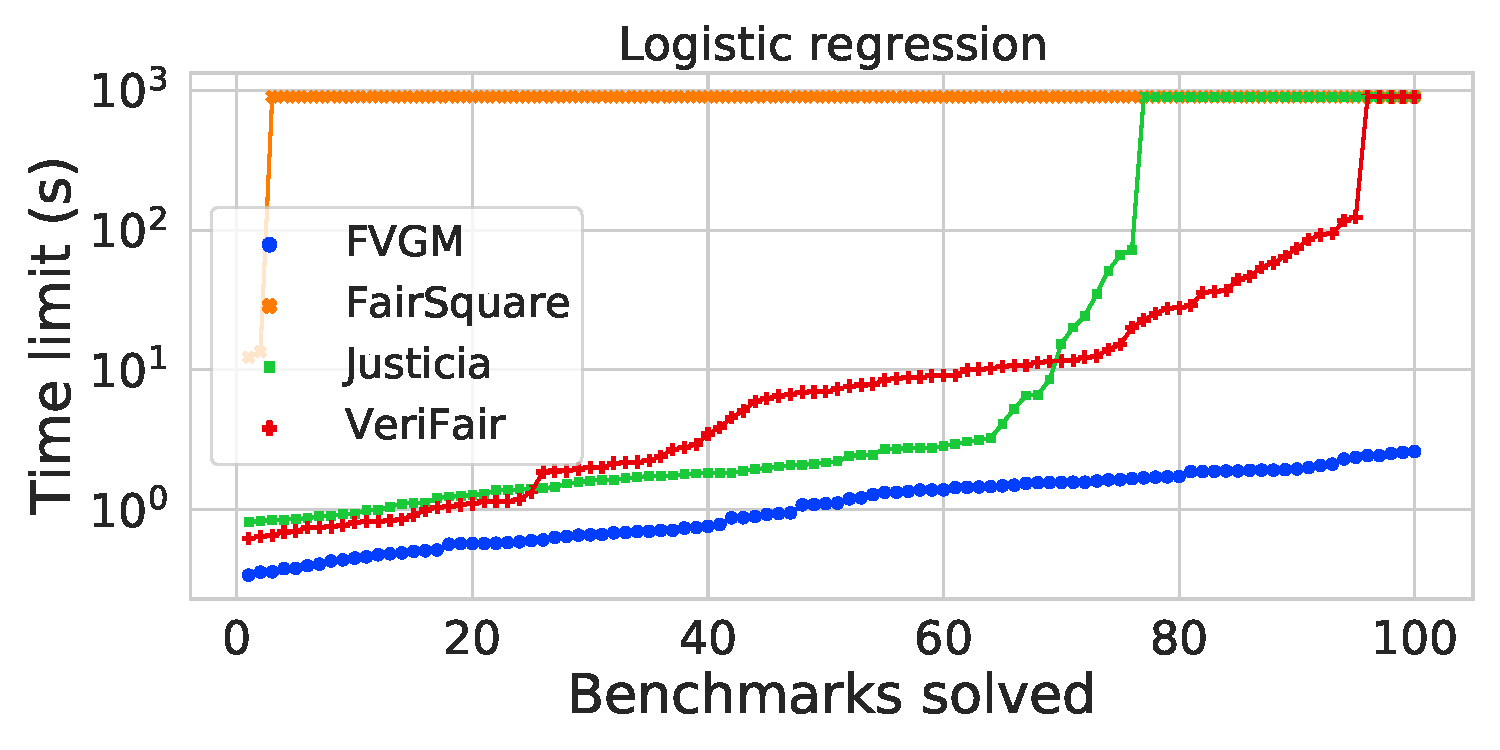
\includegraphics[scale=0.3]{figures/cactus_all_verifiers_LR_time_}
			\end{center}
			\caption{A cactus plot to present the scalability of different fairness verifiers in solving $ 100 $ fairness verification benchmarks. $ \mathsf{FVGM} $ achieves the best scalability results by solving all benchmarks with $ 1 $ to $ 2 $ orders of runtime improvement.} \label{fig:scalability_exp}
		\end{minipage}\hfill
		\begin{minipage}{0.48\textwidth}
			\centering
			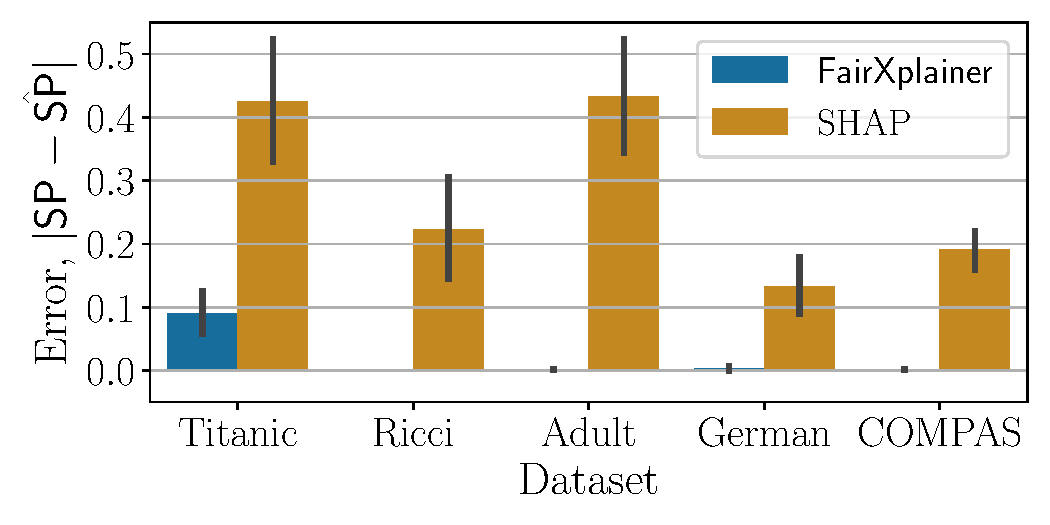
\includegraphics[scale=0.4]{figures/sp_train_accuracy}
			\caption{Comparing $ \mathsf{FairXplainer} $ and local explanation method SHAP on the estimation error of statistical parity, computed as the sum of FIFs of all subset of features~\cite{ghosh2022how}. Lower values on the $ Y $-axis denote a better result. $ \mathsf{FairXplainer} $ has significantly less estimation error than SHAP.}\label{fig:estimation_error}
		\end{minipage}
		%	\vspace{-0.5em}
	\end{figure}
	
	
	\subsection*{Research Thrust 2: Interpretable Machine Learning}

	In interpretable machine learning, rule-based classifiers are particularly effective in representing the decision boundary through a set of rules comprising input features. Examples of such classifiers include decision trees, decision lists, and decision sets. The interpretability of rule-based classifiers is in general related to the size of the rules, where smaller rules are considered more interpretable. To learn such a classifier, the brute-force direct approach is to consider an optimization problem that tries to learn the smallest classification rule achieving close to maximum accuracy. This optimization problem is computationally intractable due to its combinatorial nature and thus, the problem is not scalable in large datasets. To this end, our research goal is to study the triangular relationship among the accuracy, interpretability, and scalability of learning rule-based classifiers.
	
	\paragraph{Incremental Learning of Interpretable Classfication Rules.} We propose an incremental learning framework, called $ \mathsf{IMLI} $~\cite{ghosh22efficient,ghosh2019incremental},  based on maximum satisfiability (MaxSAT) for synthesizing classification rules expressible in proposition logic. $ \mathsf{IMLI} $ considers a joint objective function to optimize the accuracy and the interpretability of classification rules and learns an optimal rule by solving an appropriately designed MaxSAT query. Despite the progress of MaxSAT solving in the last decade, the straightforward MaxSAT-based solution cannot scale to practical classification datasets containing thousands to millions of samples. Therefore, we incorporate an efficient incremental learning technique inside the MaxSAT formulation by integrating mini-batch learning and iterative rule-learning. The resulting framework learns a classifier by iteratively covering the training data, wherein in each iteration, it solves a sequence of smaller MaxSAT queries corresponding to each mini-batch. In our experiments, $ \mathsf{IMLI} $ achieves the best balance among prediction accuracy, interpretability, and scalability. For instance, $ \mathsf{IMLI} $ attains a competitive prediction accuracy and interpretability w.r.t. existing interpretable classifiers and demonstrates impressive scalability on large datasets (Figure~\ref{fig:scalability_imli}) where both interpretable and non-interpretable classifiers fail. As an application, we deploy $ \mathsf{IMLI} $ in learning popular interpretable classifiers such as decision lists and decision sets.
	
	
	\begin{figure}[!b]
		
		\centering
		
		\subfloat[Samples: $ 32,561 $\\Features: $ 94 $]{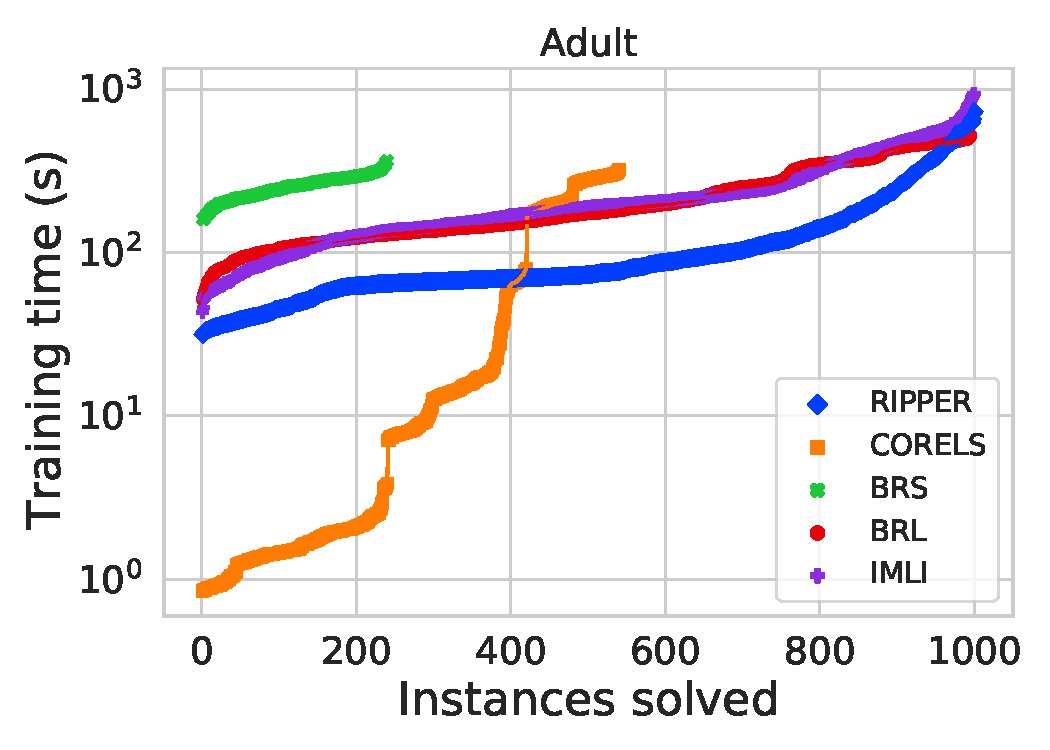
\includegraphics[scale=0.3]{figures/dataset_adult_cactus_train_val_fit_time}}
		\subfloat[Samples: $  107, 696 $\\Features: $ 169 $]{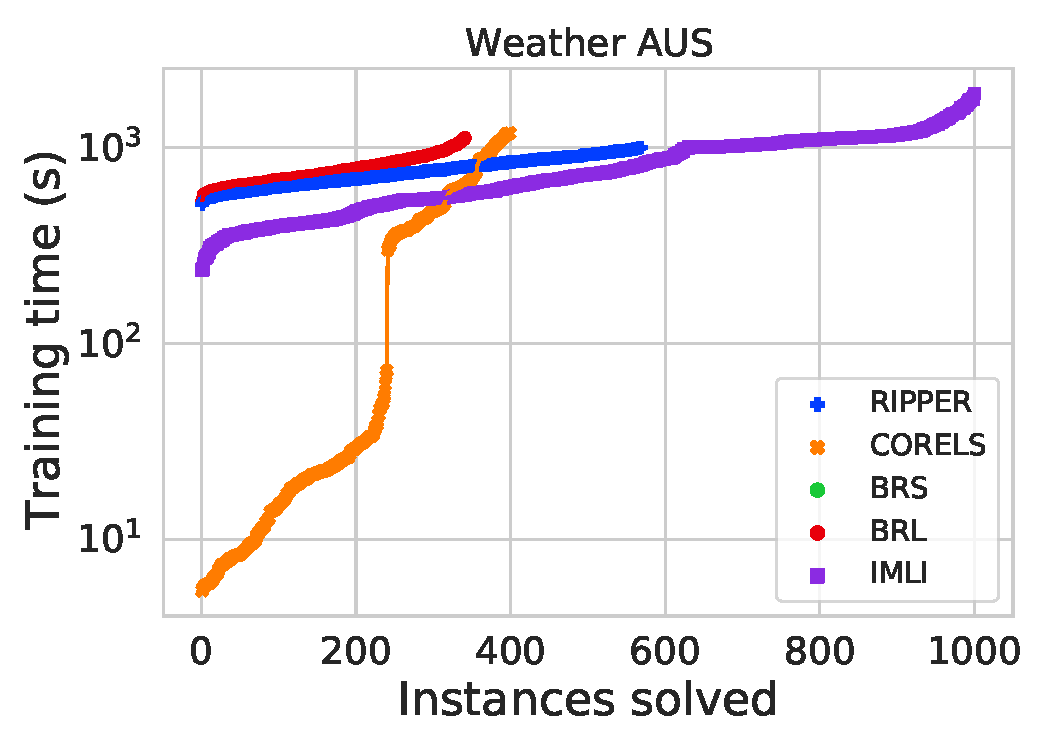
\includegraphics[scale=0.3]{figures/dataset_weatherAUS_cactus_train_val_fit_time}}
		\subfloat[Samples: $  1, 000, 000 $\\Features: $ 89 $]{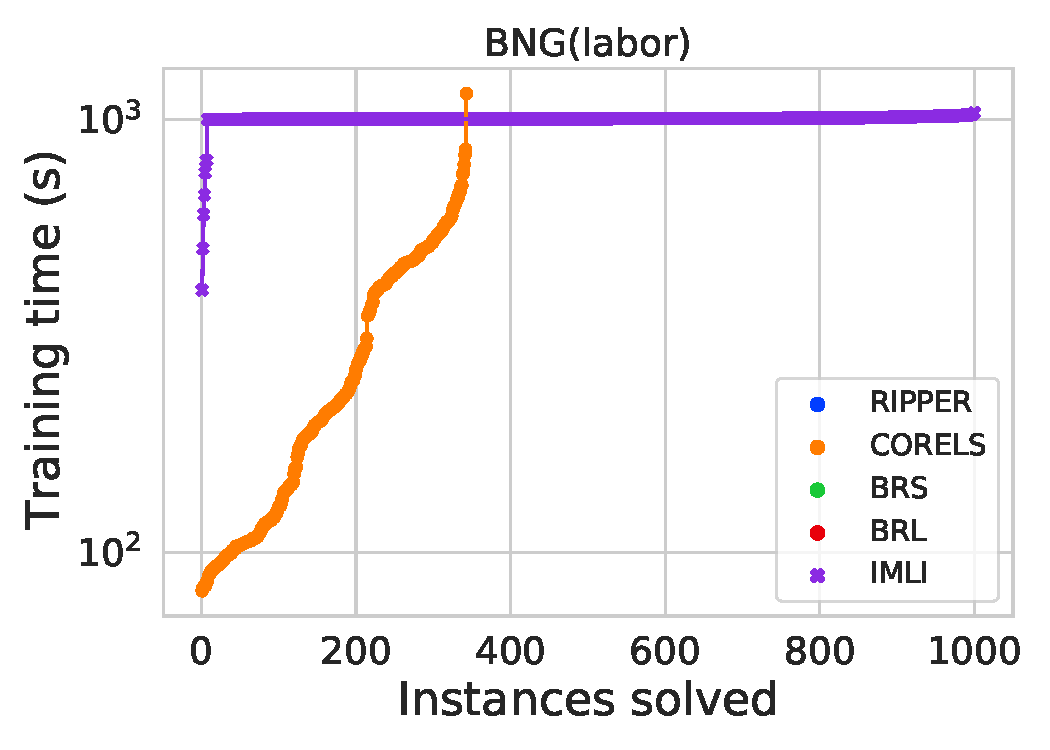
\includegraphics[scale=0.3]{figures/dataset_labor_cactus_train_val_fit_time}}
		
		\caption{Results on the scalability of $ \mathsf{IMLI} $ compared to existing interpretable classifiers, presented using cactus plots for datasets with varied dimensions. As datasets become large, $ \mathsf{IMLI} $ becomes the only interpretable classifier to classify all of $ 1000 $ classification instances for a dataset. The success of $ \mathsf{IMLI} $ is attributed to its incremental learning wrapping a MaxSAT-based formulation.}
		\label{fig:scalability_imli}
	\end{figure}
	
	
	\paragraph{Classification Rules in Relaxed Logical Form.} We extend our incremental learning framework to learn a more relaxed representation of classification rules~\cite{ghosh2020classification}. Elaborately, we consider relaxed definitions of standard OR/AND operators in Boolean logic, which allow exceptions in the construction of a clause and also in the selection of clauses in a rule. Building on these relaxed definitions, we introduce relaxed-CNF classification rules motivated by the popular usage of checklists in the medical domain. Relaxed-CNF generalizes widely employed rule representations including CNF, DNF, and decision sets. While the combinatorial structure of relaxed-CNF rules offers exponential succinctness, the na\"ive learning techniques are computationally expensive. To this end, we propose an incremental mini-batch learning procedure, called $ \mathsf{CRR} $, that employs advances in the Mixed-Integer Linear Programming (MILP) solvers to efficiently learn relaxed-CNF rules. Our experimental analysis demonstrates that $ \mathsf{CRR} $ can generate relaxed-CNF rules, which are more accurate and sparser compared to the alternative rule-based models.
	
	

	
	\section*{Future Research Plans}
	 My long-term research plan is to continue designing efficient and scalable algorithms for machine learning while prioritizing its trustworthiness in safety-critical applications. I plan to work in a collaborative environment, understand problems arising in real-world applications, and solve them with advancements in machine learning and formal methods. In the following, I discuss several research themes.
	 
	 
	 \paragraph{Fairness and Interpretability As a Service.} I envision machine learning as an alternate decision-maker of the human in the future, with applications in law, education, transportation, etc. In the high-stake and safety-critical domains, end-users expect higher transparency from black-box algorithms. Hence, achieving fairness, interpretability, robustness, and privacy are significant challenges in front of current machine learning models. While traditional machine learning such as deep learning is data-hungry, certifying safety-critical properties will be challenging in complex models and large data. From this vantage point, I aim to design efficient algorithms for the fairness and interpretability of deep models, transformer-based natural language processing (NLP), and computer vision. 
	 
	 
	 \paragraph{Counting and Optimization Problems.} My past research has been centering on formulating fairness and interpretability in machine learning as counting and optimization problems; and our proposed algorithms based on formal methods and incremental solving result in both higher scalability and better accuracy. In the future, I plan to apply these techniques in solving similar counting and optimization problems, even in areas beyond machine learning. 
	
	
	\bibliographystyle{ieeetr}
	\small{
		\bibliography{ref}
	}
\end{document}